\documentclass[a4paper]{ctexbook}

\usepackage{amsmath}
\usepackage{amsfonts}
\usepackage{booktabs}
\usepackage{graphicx}
\usepackage{multirow}
\usepackage{listings}
\usepackage{algorithmic}
\usepackage{xcolor}
\definecolor{codebg}{rgb}{0.949, 0.949, 0.922} 
\lstset{ 
	backgroundcolor=\color{codebg},
}
\usepackage[colorinlistoftodos]{todonotes}

% 定义所有的图片文件在 figures 子目录下
\graphicspath{{figures/}}

\newtheorem{definition}{\hspace{2em}定义}[chapter]

\begin{document}

\title{Web API场景建模及
\\测试自动生成的研究与实现\\{\small 本科生毕业设计}}
\author{李林翼\quad 清华大学}
\date{2018年6月10日}
\maketitle

\tableofcontents

\graphicspath{{figures/}}

\chapter{引言}

	\section{背景介绍}
    
        近年来, 云计算和移动计算获得了空前的发展, 面向服务的体系结构(SOA)已经成为了云计算和移动计算的主流架构\cite{wintergreen17}. 预计至2020年, SOA市场的规模将达到164亿美元. 而云计算业务的市场规模将于2021年达到715.5亿美元\cite{skyhighnetworks18azure}. 面向服务的体系结构经常使用web API的形式对外提供开放服务\cite{hamza15}, 这些web API常常使用SOAP(简单对象访问协议)协议或REST(表现层状态转换)风格\cite{fielding2000architectural}. Google云\cite{googlecloud17}, YouTube\cite{youtube17}, Amazon AWS\cite{amazonec217}和阿里云\cite{alibaba17}等等著名web应用均使用RESTful API作为服务接口. 一些大型公共API搜索引擎如APIs.io和百度API Store\footnote{到2017年, APIs.io(http://apis.io)数据库收录了1105项API, 而百度API Store(http://apistore.aidu.com)收录了1133项API.}均收录了超过1,000项面向web服务开发者的开放RESTful API. ProgrammableWeb平台\footnote{https://www.programmable.com/}可索引检索超过18,000项开放API.
        
        Web API常以公共服务的形式对外发布, 开发者则通过集成与组装这些web API的方法, 针对各种应用场景开发定制应用. 由于互联网应用环境的多样性和不可预测性, 在基于API的系统开发中, 缺陷和故障难以避免. API的开发者难以预见他们的API将会在什么用户场景下被用到, 更难以保证在这各种各样的环境下提供的API的绝对正确性. API的使用者也可能不熟悉API设计时对运行环境的限制, 进而很可能错误理解、错误使用这些API. 由于web API是这些上层应用的基础部件, 一旦某个web API被广泛应用, 它的任何疏漏和故障就会影响到众多应用和数以万计的用户, 甚至造成严重损失. 所以, web API的品质十分重要. 然而, web API的测试十分具有挑战性. 测试web API常常需要使用大量的测试用例来覆盖API的所有功能点和用法. 设计达到足够覆盖率的测试用例经常需要耗费大量的人力物力. 不仅如此, 由于web API实时提供、实时更新, 频繁的回归测试对于诊断和确认更新是必不可少的. 因此, 手动测试对于满足这种苛刻的web API连续集成测试而言, 是缺乏效率, 甚至是不适合采用的. 对web API进行自动化测试, 从某种意义上, 已经成为了一种必需.

	\section{研究现状}
	
    	结合我们的研究内容, 本文从三个方面考察了目前的研究现状: web API标准化, 基于模型的测试, 和自动化测试.
    	
    	在领域专用语言和软件测试的结合方面, 有一些工作已经取得了一定的进展. Anurag Dwarakanath等人\cite{dwarakanatha17}设计了一种类似于英语的领域特定语言描述UI测试的测试用例. Alex Gyori等人\cite{gyoria16}开发了NonDex工具, 对Java API规范中的错误假设条件进行检测和修正. 在单API测试中, Andrea Arcuri\cite{andreaa17}应用遗传算法来为使用OpenAPI规约语言编写的RESTful API自动生成测试用例. OpenAPI\cite{openapi17}是一种描述RESTful web API的行为的广受欢迎的领域特定语言, 我们的方法也基于OpenAPI. Ruben Verborgh和Michel Dumontier\cite{verborgh2016web}讨论了在基于功能的web API复用中, Swagger(OpenAPI的曾用名)规约所起到的关键作用. Erik Wittern等人\cite{wittern2017statically}从GitHub中挖掘代码仓库, 然后使用OpenAPI规约自动检查JavaScript编写的API请求与标准的一致性. Swagger Inspector\cite{swaggerinspetor17}工具支持基于规约的简单API测试, 但是多API的集成测试方面, 它仅仅支持发送单一序列请求.
    	
    	基于模型的测试是测试自动化的重要研究方向. 近年来, 已经提出了许多模型和基于模型的软件测试技术. James A. Whittaker\cite{Whittaker1997}综述了马尔科夫模型及其随机性质在软件测试中的应用. Alan Jorgensen和James A. Whittaker\cite{jorgensen2000api}总结并提出了API测试的类型分区和马尔科夫建模测试法. 概率有限状态自动机(PFSA)\cite{enriquev05}是一种形式化定义的自动机模型, 它已经在软件建模和分析中得到了一定应用. 本文也将使用它作为场景模型的基础模型. Anand Raman和Jon Patrick\cite{anand97}提出了一种从序列分布中建模出对应PFSA模型的快速算法. 此算法扩展自一些更早期的工作, 如A. W. Biermann和J. A. Feldman提出的k-tails方法\cite{abiermann72}. 王钧奕等人\cite{junyiw17}在他们开发的分布式web API测试工具中使用了概率转移图模型. 他们的工具可以自动生成请求序列, 但是忽略了数据流依赖. Hung Viet Pham等人\cite{pham2016learning}提出了基于图的API调用场景表示和可从字节码中学习的API调用统计生成模型. 此外, Cyrille Artho等人\cite{cyrille17}在Apache ZooKeeper的API测试中使用了事件图模型. Robert Feldt和Simon Poulding\cite{feldt2017searching}总结出, 统计模型是一种生成特征多样化测试数据的重要方法.
    	
    	在自动化测试方面, 随着面向服务的体系架构和web API的日益流行, web API的自动化测试日益成为研究热点. 在自动化生成API请求序列方面, 谢涛和裴健\cite{taox06}开发了MAPO工具, 此工具之后由钟浩进一步扩展\cite{Zhong2009}, 该工具融合了数据挖掘与代码分析方法, 可以挖掘与发现出API的频繁调用序列. 在此之后, Jaroslav Fowkes和Charles Sutton\cite{fowkes2016parameter}提出了PAM(概率式API挖掘器)算法, 这是一个几乎无需参数设置的API调用模式挖掘的概率式算法. 相比于MAPO, PAM在提取GitHub的相关API调用序列方面要明显更优. 循环神经网络(RNN)在序列建模方面十分有用. Junyoung Chung等人\cite{chung2014empirical}评估了很多不同类型的RNN单元在序列建模任务上的表现. 最近, 顾小东等人\cite{xiaodongg16}提出了一种用于API序列和依赖建模的基于RNN的自然语言模型. 在我们之前的工作中, 侯可佳等人\cite{kejiah13}分析了API序列的数据依赖和约束. 它们开发了进行自动化测试数据分区与生成的工具框架. 
    	
    	关于RESTful API的开发模式, Micheal Stowe\cite{michaels15}, Leonard Richardson和Sam Ruby\cite{leonardr07}讨论了规约驱动的RESTful API开发方式.
    	
    	Web API的场景模型, 在本文中主要用于自动化生成, 其实还可作为API用户的有效API使用指南, 和API设计者的设计分析参考. Brad A. Myers等人\cite{bradm17}讨论了对API设计者, 开发者和用户而言, 提高API易用性的重要性.

	\section{研究内容和结构安排}
	
	    本文的课题分为两个主要方面: 场景建模与测试生成.
	
	    在场景建模方面, 本文提出了一种描述API调用行为的场景模型. 我们的模型基于概率有限状态自动机(PFSA)而扩展, 以支持测试数据与约束的表达. 其中, 一个API服务端点被建模为一个自动机的状态. 每个包含端点的状态定义了附着的请求数据约束集合, 响应断言集合. 每个状态转移上定义了触发的条件约束. 带权值的状态转移边则建模了执行相应服务端点后, 进行相应状态转移的概率. 目前, 具体的场景模型需要手动设计. 但场景模型的状态, 约束, 断言, 和转移边的概率分布等各个组件均可能从历史记录和日志中自主学习生成.
	
        在测试生成方面, 本文主要提出了一种基于场景模型的web API自动化测试方法. 给出使用标准规约格式表达的场景模型, 本文提出的算法可以自动生成测试请求数据, 并遍历生成测试请求序列.
        
        \begin{figure}[htbp]
            \centering
            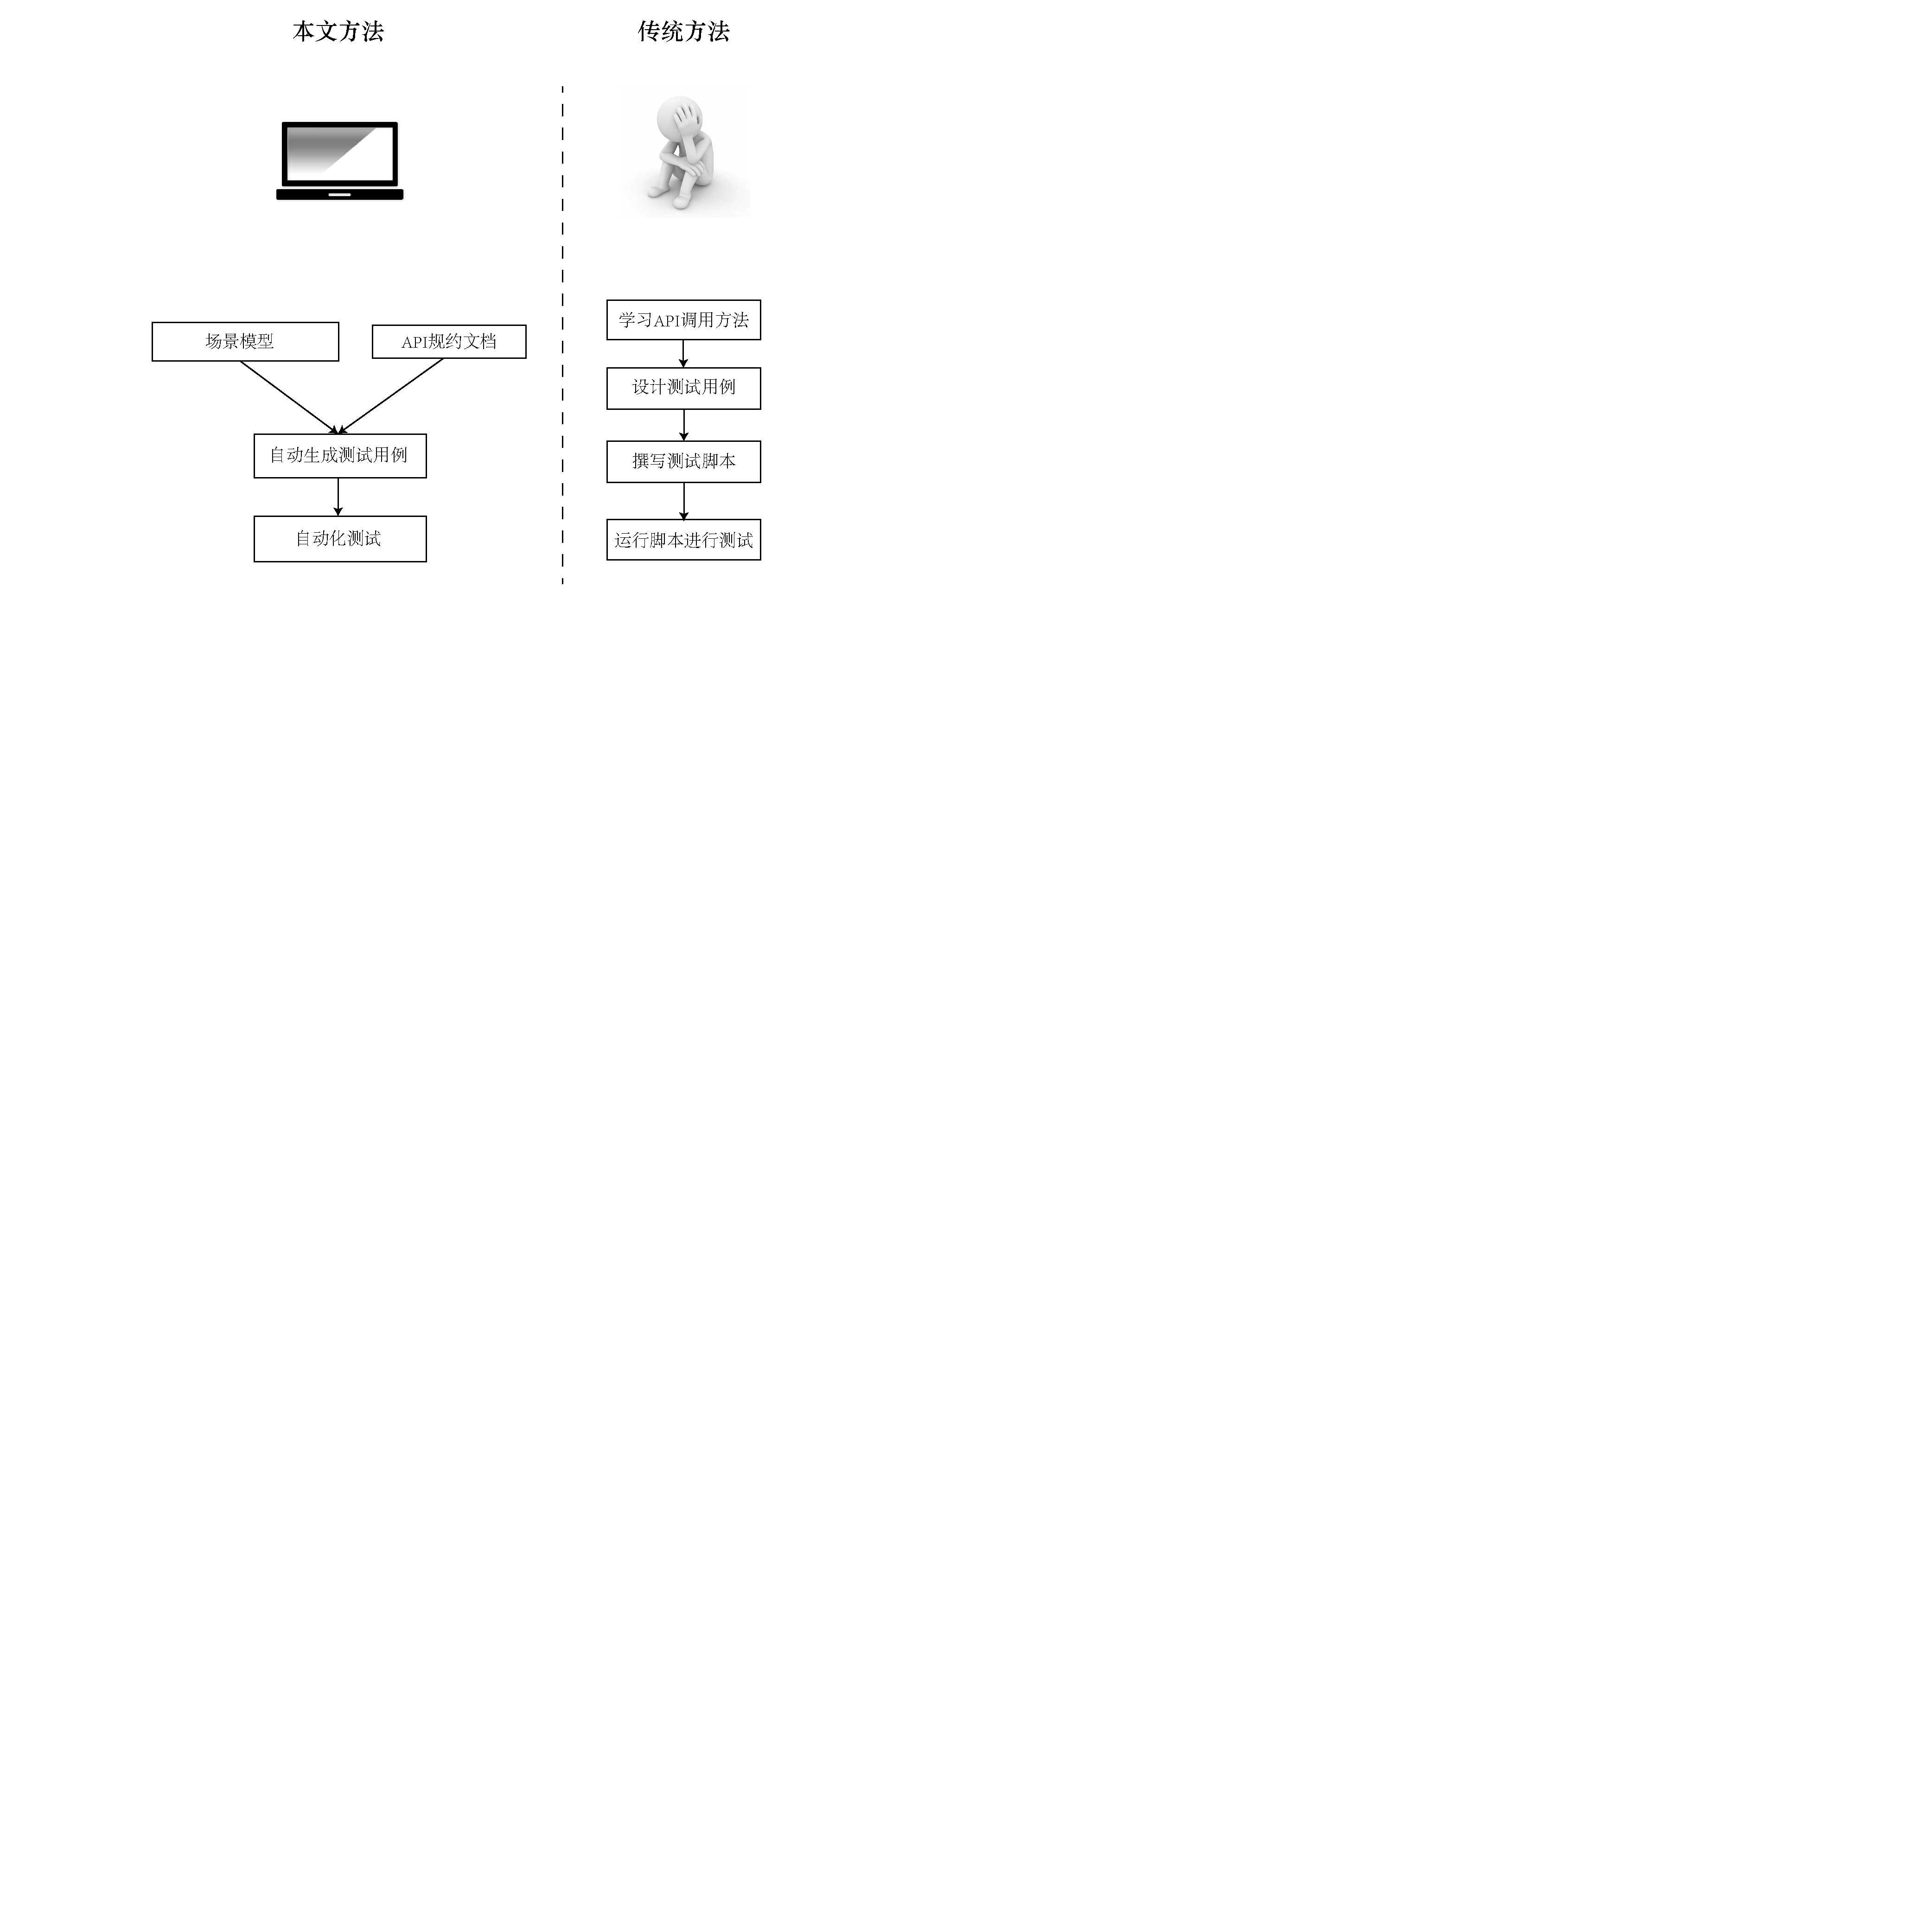
\includegraphics[width=300pt]{work_role_partial.pdf}
            \caption{本文方法与传统方法的对比. 在本文的方法中, 由于API规约文档已经提供, 人工参与的部分仅有场景设计, 其余部分均完全自动化. 而在传统方法中, API调用方法的学习, 测试用例的设计, 以及测试脚本的撰写, 均需要大量人力付出.}
            \label{fig:overview}
        \end{figure}
        
        图\ref{fig:overview}展示了本文提出的自动化测试方法的总体框架, 并将其与传统人工方法进行了对比. 如图中右半部分所示, 在传统方法中, 手工测试员首先需要学习API的调用请求方法, 然后设计测试用例, 撰写测试脚本, 并手动运行测试脚本. 这个过程需要大量的人力付出, 并且冗长无聊, 耗时耗力. 而且, 测试的品质在很大程度上依赖于测试员的经验和水平.
        
        为了应对这些困难, 本文提出了一种自动化测试方法, 并实现了原型工具Lapis. 本文的自动化方法旨在以下方面改进传统的测试方法:
        \begin{itemize}
            \item 测试设计. \\
                在本文的方法中, 测试员只需要设计使用场景, 而不再是具体的每个测试用例. 本文的场景模型可以有效描述web API的控制流与数据流约束, 测试断言以及频繁使用模式. 相比直接设计测试用例, 由于一个测试场景可以自动生成多种各不相同的测试用例, 因此设计测试场景可有效节约设计成本.
            
            \item 测试生成.\\
                在本文的方法中, 测试用例是由场景模型直接生成的. 使用本文提出的多种模块化测试数据生成算法和API调用序列生成算法, 测试用例的质量可以很容易地得到保证和提高. 并且, 由于实现了自动化, 测试用例的数量也可以远远超过手动设计的数量.
            
            \item 测试执行.\\
                目前已有的规约格式, 如OpenAPI, 提供了对RESTful API的详细形式化定义. 定义的组件包括了调用协议, 主机地址, 各个参数的格式和响应体的格式等等. 因此, 一旦有了测试数据, 便可以实现自动发送请求和相应解析. 在本文的方法中, 我们应用了OpenAPI来实现这一功能, 将手工测试员从书写API调用脚本的繁重劳动中解放了出来.
        \end{itemize}
        本文介绍的原型工具Lapis, 即实现了此自动化方法, 包括规约导向的API分析, 使用场景模型解析, 测试用例生成和测试用例执行等.
        
        本文的结构安排如下: 第二章介绍基本模型与方法, 包括形式化的场景模型, 和基于模型的测试数据与测试用例生成方法, 以及如何对生成的测试场景进行以故障检测为导向的优化. 第三章介绍原型系统的设计与实现, 包括原型系统的整体概述, 方法的具体实现等. 第四章展示原型系统在实际API服务上的实验结果, 并进行了实验结果的初步分析. 第五章进行总结, 并讨论了未来可继续进行的研究方向.
        


\chapter{场景建模与测试生成方法}
    \section{场景模型定义}
        \textbf{使用场景模型}是一种有效的模型化技术. 使用场景模型可以描述在现实世界中, 一或多个人如何与系统进行交互\footnote{http://agilemodeling.com/artifacts/usageScenario.htm}. 模型包括了交互过程中的步骤, 事件和动作. 本文提出了一种描述与web API的交互的使用场景模型. 为了基于模型进行测试生成, 模型着重于抽象以下web API的特点:
        
        \begin{itemize}
            \item 与使用场景相关的服务的元素. 这包括服务的功能, 请求数据, 响应数据, 执行约束等.
            
            \item 交互中, 各服务之间的交互. 这包括执行序列和序列内通信, 比如调用序列中之前某个服务的响应, 可能作为之后调用其他服务的参数.
            
            \item 不同交互操作的频率. 在有限测试资源的情况下, 对于测试资源的分配, 各个被测API需要有优先级顺序. 比如, 一些API可能在许多场景下都被用到, 被频繁地调用, 或者为许多其他API提供前置服务. 那么, 根据基于使用的测试原则, 这些频繁使用的API需要进行更多测试. 因此, 对API使用的分析与建模有助于优化对各个API和场景所生成的测试用例数量.
        \end{itemize}
        
        概率有限状态自动机(PFSA)可以有效描述相关服务, 执行序列和交互频率. 然而, 对于数据约束和服务通信, 它的能力有所不足. 我们的模型基于概率有限状态自动机进行扩展, 克服了这些不足.
        
        \subsection{背景: 概率有限状态自动机}
        
            概率有限状态自动机(PFSA)是非确定性有限状态自动机(NFA)的扩展. 它对非确定性有限状态自动机的转移, 起始状态和终止状态加入了概率因素. 对于每个串中读入的字符, 自动机会根据从当前状态出发的转移边的概率分布, 来从可选的转移边中选择一项进行转移. 状态的初始化和终止也具有类似的概率性质.
            
            根据Enrique Vidal等人的阐述\cite{enriquev05}, 一个基本的概率有限状态自动机具有如下的定义(定义\ref{def.pfsa}).
            
            \begin{definition}
                \label{def.pfsa}
                概率有限状态自动机为一个元组
                \begin{equation}
                    \mathcal{B} := <Q_{\mathcal{B}}, \Sigma, \sigma_{\mathcal{B}}, I_{\mathcal{B}}, F_{\mathcal{B}}, P_{\mathcal{B}}>,
                \end{equation}
                
                其中:
                \begin{itemize}
                    \item $Q_{\mathcal{B}}$是有限的状态集合;
                    \item $\Sigma$是字符集;
                    \item $\sigma_{\mathcal{B}} \subseteq Q_{\mathcal{B}} \times \Sigma \times Q_{\mathcal{B}}$是状态转移的集合;
                    \item $I_{\mathcal{B}} : Q_{\mathcal{B}} \to \mathbb{R}^{+}$是各个状态作为起始状态的概率分布;
                    \item $P_{\mathcal{B}} : \sigma_{\mathcal{B}} \to \mathbb{R}^{+}$是各个转移边的转移概率;
                    \item $F_{\mathcal{B}}: Q_{\mathcal{B}} \to \mathbb{R}^{+}$是于各个状态处终止的概率分布.
                \end{itemize}
                
                $I_{\mathcal{B}}$函数满足初始状态概率归一化性质:
                \begin{equation}
                    \sum_{q \in Q_{\mathcal{B}}} I_{\mathcal{B}}(q) = 1.
                \end{equation}
                
                $P_{\mathcal{B}}$和$F_{\mathcal{B}}$函数满足转移概率归一化性质:
                \begin{equation}
                    \forall q \in Q_{\mathcal{B}}, F_{\mathcal{B}}(q) + \sum_{a \in \Sigma, q' \in Q_{\mathcal{B}}} P_{\mathcal{B}}(q,a,q') = 1.
                \end{equation}
            \end{definition}
            
            按照惯例, 概率有限状态自动机使用带标签边的有向图表示. 图\ref{fig:PFSA_example}展示了一个概率有限状态自动机的例子. 其中, 图的节点表示自动机的状态, 图的带标签边表示自动机的概率转移边, 图的节点数字表示自动机状态的终止概率.
            
            \begin{figure}
                \centering
                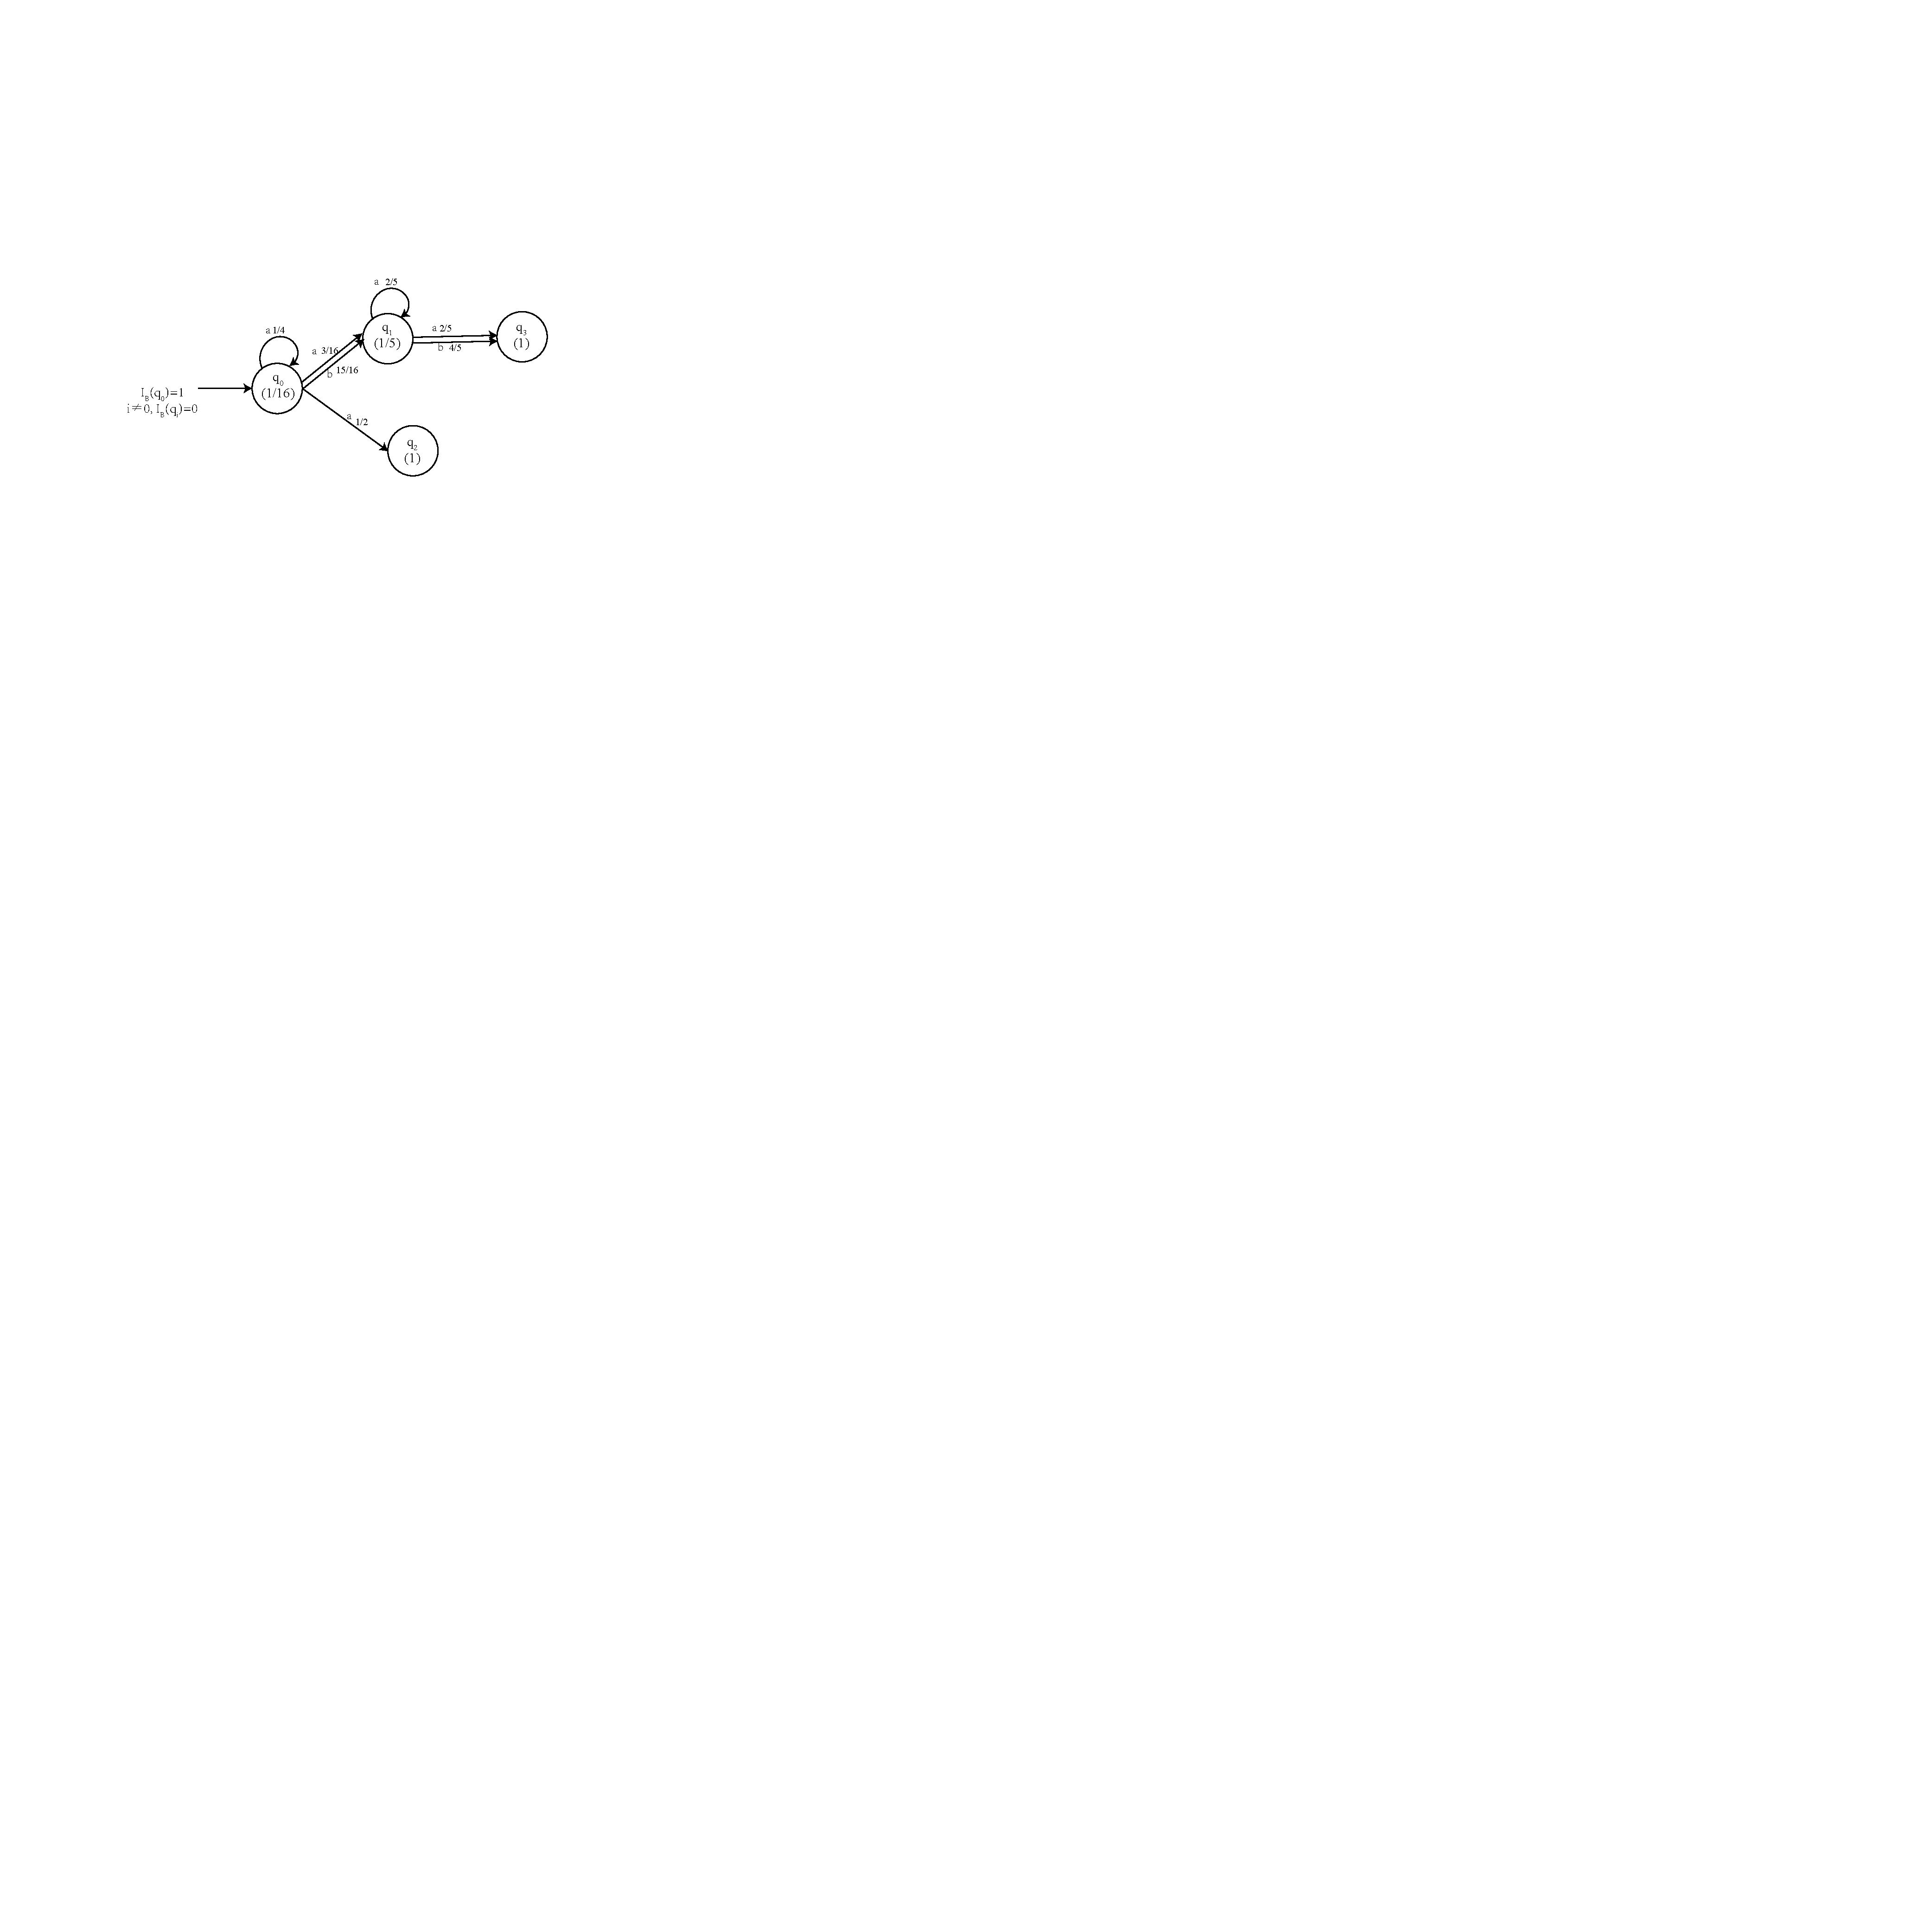
\includegraphics[width=300pt]{PFSA_example.pdf}
                \caption{概率有限状态自动机的可视化表示}
                \label{fig:PFSA_example}
            \end{figure}
            
            概率有限状态自动机是一种随机模型, 它生成的是在有限串集合$\Sigma^{*}$上的概率空间. 对于此自动机, 生成一个串的步骤为:
            
            \begin{itemize}
                \item 初始化: 按照概率分布$I_\mathcal{B}$选择一个$Q_{\mathcal{B}}$中的状态$q_0$作为初始状态;
                
                \item 生成: $q$表示当前状态. 以$F_{\mathcal{B}}(q)$的概率决定是否在此状态处终止, 或者以$P_{\mathcal{B}}(q, a, q')$的概率决定是否进行转移$(q,a,q')$. 如果进行此转移, 则输出$a$并将$q'$置为当前状态.
            \end{itemize}
        
            概率有限状态自动机的以下特点让其适用于使用场景的建模:
            
            \begin{itemize}
                \item 自动机的状态可以很方便地与服务端点关联起来. 因此, 状态的转移可对执行序列进行建模.
                
                \item 自动机的字符集$\Sigma$可建模服务端点的所有可能的响应. 另一方面, 每个状态转移均对应一个字符$c \in \Sigma$, 其表示此转移仅适用于当前读入字符为$c$的情形. 因此, 这个对应字符可建模各个转移所适用的范围, 此范围由服务端点的返回响应决定. 也就是状态转移对应的字符定义了进行此状态转移的条件.
                
                \item 自动机的起始概率, 终止概率, 转移概率反映了进行不同交互的频率差异.
            \end{itemize}
            
            然而, 在使用场景模型中关键的数据约束, 数据依赖, 测试断言则很难在概率有限状态自动机中表达与反映. 本文的场景模型扩展了概率有限状态自动机模型来克服这些问题.
        
        \subsection{模型定义}
            本文的场景模型在以下方面扩展了基本概率有限状态自动机:
            
            \begin{itemize}
                \item 它在状态定义中加入了请求数据约束与请求数据依赖的定义, 以便于生成请求数据.
                
                \item 它在状态定义中加入了响应数据约束与测试断言 的定义, 以便于对响应进行验证.
            \end{itemize}
            
            形式化的定义如下:
            
            \begin{definition}
                \label{def:our}
                场景模型是一个元组
                \begin{equation}
                     \mathcal{A} := <Q_{\mathcal{A}}, \Sigma, \sigma_{\mathcal{A}}, I_{\mathcal{A}}, F_{\mathcal{A}}, P_{\mathcal{A}}>,
                \end{equation}
                
                其中:
                \begin{itemize}
                    \item TODO
                \end{itemize}
            \end{definition}
        
        \subsection{解释与说明}
        
        \subsection{示例}
    
    \section{测试生成方法}
    
    \section{*测试场景优化}


\chapter{原型系统设计与实现}

	\section{系统结构}

	\section{脚本解析模块}

	\section{测试生成模块}

	\section{用户接口}
		\subsection{编程接口}

		\subsection{web端脚本编辑系统}

		\subsection{*桌面端测试管理系统}



\chapter{实验与评估}
    \label{sec:experiment}

    本工作的原型系统在三个实际的web API服务上进行了实验, 从四个方面评估了本文提出的场景模型和测试方法: 测试用例多样性, 测试覆盖率, 故障检测能力, 以及测试效率.
    
    \section{实验配置}
        实验选择的第一个被测系统为合作研究组开发的云对象存储服务(OSS)的系统原型(后文简称\textbf{OSS}). 此服务提供了33个web API接口, 并有较完整的使用文档. 测试时, 期望所有的API和功能点都业已实现完成.
        
        最近以来, 云对象存储服务(OSS)已经成为了流行的云存储服务形式. 许多大型云服务提供商均已提供云对象存储服务, 如亚马逊AWS\footnote{https://aws.amazon.com/s3}, IBM云\footnote{ https://console.bluemix.net/catalog/services/cloud-object-storage}和阿里云\footnote{ https://www.alibabacloud.com/product/oss}等. 在云对象存储服务中, 每个账号, 在每个服务器区域, 都可以有许多桶(bucket). 桶(bucket)与文件系统中的文件夹类似, 对象(object)与文件系统中的文件类似. 用户可以上传对象, 删除对象, 重命名对象, 创建符号链接等等. 每个对象都属于一个固定的桶.
        
        对于云对象存储服务, 本工作首先为这33个API编写了OpenAPI格式的API行为描述脚本. 然后, 设计了一些小型场景模型来检验每个API的基本功能. 在此之后, 设计了三个较大型的综合场景模型Scenario A(详见附录图\ref{fig:oss_scenario_A})、Scenario B(详见附录图\ref{fig:oss_scenario_B})、Scenario C(详见附录图\ref{fig:oss_scenario_C})以进行综合测试, 这三个场景均与实际使用场景较相似, 测试用例的生成与执行期望能够模拟实际部署后的高负载环境. 对于每个场景, 运行工具原型随机生成并执行了1,000个测试用例. 所有测试用例及其执行结果都被妥善保存. 后续分析时, 在所有测试用例上进行统计, 而没有进行任何遴选.
        
        第二个被测系统为阿里云的云服务器(ECS)服务(后文简称\textbf{ECS}), 阿里云是世界领先的云计算服务商, 淘宝、12306网站等大型应用均依托阿里云提供计算支持. 
        
        本实验测试阿里云服务为普通用户提供的云计算实例租用服务, 相关接口共有26个, 均为web API, 并配有专业使用文档. 在此服务中, 用户可以租用示例, 退租示例, 获取实例运行状态, 启动示例, 关闭示例, 重启示例等等. 我们选择了其中8个web API, 编写了行为描述脚本, 然后设计了包含所有这8个web API的综合场景模型(详见附录图\ref{fig:ecs_scenario})进行测试. 一共随机生成并执行了100个测试用例, 所有测试用例在进行统计与分析时均纳入考虑.
        
        第三个被测系统是工业界合作团队提供的电子支付服务(后文简称\textbf{E-payment}). 本实验测试它的实时贷记API接口. 此API仅用于系统内部使用, 是微服务之间的通信接口, 因此使用LAN上的定制协议交互. 作为电子支付接口, 此服务拥有很高的可用率与很低的容错率要求. 同时, 它有多达20个参数. 由于模拟环境的缺失, 在本实验中, 暂未进行实际的调用与发送, 而是根据接口描述文档进行测试用例和请求数据的生成, 来验证生成的测试用例可以有效覆盖参数组合, 从而验证其在这类服务的测试上的可用性.
        
        对于E-payment服务, 实验中生成了巨量(超过两百万个)的测试用例, 并计算了这些测试用例对于参数组合的覆盖率. 这种方式不仅仅评估了测试用例的覆盖率, 也检验了工具原型的鲁棒性和性能. 使用的场景主要进行基于数据分区的请求参数生成和参数合成操作, 详见附录图\ref{fig:epayment_scenario}.
        
    
    \section{测试用例多样性}
        富有多样性的测试用例是本文测试方法追求的目标之一. 多样性保证了测试用例集构成的测试套件具有较高的覆盖率和较低的冗余度. 另一方面, 使用被测系统的用户形形色色, 实际的系统负载也十分富有多样性, 因此, 测试用例富有多样性, 在某种程度上也能说明生成它们的测试场景模型可以很好地表达使用场景.
        
        \begin{figure}[!htb]
            \begin{minipage}{0.5\textwidth}
                \centering
                \includegraphics[width=200pt]{OSS_A_APICalls_cn.pdf}
                \includegraphics[width=200pt]{OSS_B_APICalls_cn.pdf}
                \includegraphics[width=200pt]{OSS_C_APICalls_cn.pdf}
            \end{minipage}
            \begin{minipage}{0.5\textwidth}
                \centering
                \includegraphics[width=200pt]{OSS_A_UploadedObj_cn.pdf}
                \includegraphics[width=200pt]{OSS_B_AclChange_cn.pdf}
                \includegraphics[width=200pt]{OSS_C_Putsymlink_cn.pdf}
            \end{minipage}
            \caption{OSS测试用例操作次数统计直方图. 基于Scenario A, Scenario B, Scenario C三个场景生成的1,000个测试用例. 左侧为每个测试用例调用API的总次数直方图, 右侧对每个场景选取一种典型API, 统计其调用次数直方图.}
            \label{fig:OSS_stat}
        \end{figure}
        
        \begin{figure}[!htb]
            \centering
            \includegraphics[width=200pt]{EC_instance_distribution_cn.pdf}
            \caption{ECS测试用例实例创建数直方图. 基于ECS测试场景生成的100个测试用例.}
            \label{fig:ECS_stat}
        \end{figure}
        
        在web API测试中, 测试用例的多样性可以通过很多不同的指标反映出来. 图\ref{fig:OSS_stat}反映了对于OSS服务, 生成的测试用例的总API调用次数和典型单API调用次数的统计分布情况. 图\ref{fig:ECS_stat}反映了对于ECS服务, 生成的测试用例创建的实例数的统计分布情况. 虽然由于不同API在场景中所处位置不同的原因, 每副直方图中的分布区间差异较大, 但是整体分布模式是类似的, 即无论是API总调用数目, 单API调用数目, 还是实例创建数目, 分布均较分散. 这反映了生成的测试用例的多样性.
        
        值得注意的是, 虽然这些直方图反映的分布都与指数分布较为接近, 但这只是因为, 在这些场景中大体模式均为一个总状态连接到调用各API的分状态, 并拥有不为零的终止概率, 因此测试用例中各API的调用次数才近似于指数分布. 对于其他场景模式, 其余分布模式当然是完全可能出现的.

    \section{测试覆盖率}
        覆盖率是软件测试中的一项重要指标. 存在许多类型的覆盖率. 在规范导向的黑盒API测试中, 没有办法获取源代码. 因此, 基于源代码的代码覆盖率指标和分支覆盖率指标无法使用. 此处使用的覆盖率指标主要为API覆盖率和数据分区组合覆盖率.
        
        \subsection{API覆盖率}
        
            本文中, 定义某个API的覆盖率为, 在所有生成的测试用例中, 覆盖了这个API的测试用例个数与测试用例总数的比例. 在OSS系统的实验中, 对每个场景模型包含的API服务均计算了API覆盖率. 其中, Scenario B和Scenario C场景的API覆盖率十分理想. 除了“DeleteBucketLogging”这项API只被57.1\%的测试用例覆盖外, 所有其他API的覆盖率均超过了90\%.
            
            然而, 在Scenario A中, “DeleteBucketWebsite”, “DeleteMultipleObject”和“DeleteBucket”的API覆盖率均不足20\%, 尤其是“DeleteBucketWebsite”的覆盖率为0. 仔细研究这个现象后, 发现这是由被测系统的一个故障引起的: 在请求了“PutBucketWebsite”之后, 对于其他关于对象和网页设置的操作, 被测系统变得极易崩溃. 特别是, 在请求了“PutBucketWebsite”之后, 请求“GetBucketWebsite”一定会导致系统崩溃. 但是, 在场景中如果要经过与“DeleteBucketWebsite”关联的状态, 则一定会在之前经过与“GetBucketWebsite”关联的状态, 而在请求“GetBucketWebsite”之前又一定会请求“PutBucketWebsite”. 因此, 在到达与“DeleteBucketWebsite”关联的状态时, 被测系统已经崩溃, 测试用例的执行已经结束. 实际上, 在Scenario A中一共只有8.5\%的测试用例是正常结束的, 而在无崩溃现象的Scenario B和Scenario C中所有测试用例均能正常结束.
            
            以上实验结果表明, 本文提出的场景模型, 在OSS服务中可以有效覆盖被测API服务. 另外, 某一API的异常低覆盖率很大程度上可以表征此API具有故障.
        
        \subsection{数据分区组合覆盖率}
        
            \label{sec:partition}
            
            组合测试策略\cite{grindal2005combination}是一种根据组合策略, 它对测试的不同输入参数进行组合, 来生成测试用例.
            
            在E-payment服务中, 实时贷记业务的API接口具有多于20个参数. 每个参数的可能取值, 包括合法取值与非法取值, 可以被划分为一些互不相交的集合. 本文对E-payment服务测试时, 共考虑了13个参数的数据组合, 把每个参数的取值集合划分为2-5个分区,  它们的全组合共有1,152,000种. 评估指标为数据分区组合覆盖率, 即生成的测试用例总共覆盖的数据分区组合百分比. 此覆盖率越高, 数据分区的组合被覆盖得越全, 测试效果越好. 
            
            本文提出了一种进行组合测试的场景模型模式, 详见附录\ref{sec:epayment_scenario_model}. 在此模式中, 每个非最末状态进行基于数据分区的单参数生成, 最末状态组合之前的单参数, 对被测系统发送请求体. 使用此模式, 便可在本文的场景模型上运用组合测试策略.
            
            \begin{figure}[!hbp]
                \centering
                \includegraphics[width=200pt]{webank1_cn.pdf}
                \includegraphics[width=200pt]{webank2_cn.pdf}
                \caption{测试分区数 - 生成用例数关系图. 图中, 实线表示实验结果; 青色虚线为$y=x$, 表示最理想情况, 即每个生成用例贡献一个新数据分区覆盖; 黑色虚线表示数据分区总数.}
                \label{fig:partition}
            \end{figure}
            
            实验共生成了逾200万个测试用例, 生成的测试用例数目与总共覆盖的分区组合数目的关系如图\ref{fig:partition}所示. 在图中, 青色虚线表示最理想的测试用例生成方法, 即每个新生成的测试用例均覆盖一个新的数据分区; 黑色虚线表示数据分区的总数(1,152,000); 蓝色实现表示在本文的场景模型上运行组合测试策略的实验结果.
            
            当生成的测试用例数为总数据分区组合数(1,152,000)时, 覆盖的数据分区组合数为728,239, 数据分区组合覆盖率为63.2\%. 当测试用例数为总数据分区组合数的两倍时, 覆盖数增加至996,642, 对应覆盖率为86.5\%. 此结果说明, 使用本文的场景模型运行组合测试策略时, 如果生成测试用例数与总数据组合数为同一数量级, 测试用例便可以覆盖大部分数据组合, 因此是十分有效的. 理论推导亦可推出此结论(详见附录\ref{sec:partition_deduction}).
    
    \section{故障检测能力}
    
    \section{测试效率}


\chapter{总结与展望}
    \section{与相关工作的对比}
        本文提出了描述web API使用的场景模型, 与基于它的自动化测试方法. 目前, 在web API的自动化测试领域, 亦有类似研究. 本小节将本工作与学术界相关工作、工业界仍普遍采用的手工脚本测试法, 从表达控制流能力、表达数据流能力以及测试用例多样性方面, 进行了简要对比.
    
        具体来说, 考虑以下3种测试方法作为对比:
        \begin{itemize}
            \item 概率转移图\cite{junyiw17}: 此模型使用有向图表示. 在图上进行遍历, 并根据出边的权值概率性地选择下一节点, 便可以自动化地生成测试用例.
            
            \item 请求序列: 文献\cite{taox06}\cite{xiaodongg16}中, 通过静态分析和数据挖掘方法, 从开源仓库中获得API请求序列的频繁模式. 这种序列可以使用标准化格式编码, 并导入Swagger Inspector工具\cite{swaggerinspetor17}执行.
            
            \item 测试脚本: 在工业界的企业中, 最常见的仍然是使用测试人员手工编写的测试脚本.
        \end{itemize}
        
        \begin{table}
            \centering
            \begin{tabular}{c|c}
                 &  \\
                 & 
            \end{tabular}
            \caption{Caption}
            \label{tab:related_work_compare}
        \end{table}
        
        表\ref{tab:related_work_compare}对这些不同方法进行了对比.




%% 参考文献
% 注意:至少需要引用一篇参考文献,否则下面两行可能引起编译错误。
% 如果不需要参考文献,请将下面两行删除或注释掉。
% 数字式引用
% \bibliographystyle{thuthesis-numeric}
% 作者-年份式引用
% \bibliographystyle{thuthesis-author-year}

\bibliographystyle{plain}
\bibliography{ref/refs,ref/appendix1bib}

\end{document}
